After rigorously defining what language models are (and what they are not) and learning how we can estimate them, it is time to finally introduce concrete models with which we will model language.
In this section, we introduce one of the simplest classes of language models---those that only take into account a finite context of history when modeling the conditional distribution of the next possible symbol.

\subsection{Weighted Finite-state Automata}

As we will see, finite-state language models are conveniently formalized using weighted finite-state automata.
We, therefore, begin by briefly reviewing the theory of finite-state automata with real-valued weights. 
In words, finite-state automata are one of the simplest devices for defining a formal language. 
We give a formal definition below.
\begin{definition}[Finite-state Automata]
A \defn{finite-state automaton} (FSA) is a 5-tuple $\fsatuple$ where 
\begin{itemize}
    \item $\alphabet$ is an alphabet;
    \item $\states$ is a finite set of states;
    \item $\initial \subseteq \states$ is the set of initial states; 
    \item $\final \subseteq \states$ the set of final or accepting states;
    \item A finite multi-set $\trans \subseteq \states \times \left( \alphabet \cup  \set{\eps} \right) \times \states$.\footnote{The fact that it is a multi-set reflects that it can contain multiple copies of the same element (i.e., transitions between the same pair of states with the same symbol).}
    Elements of $\trans$ are generally called \defn{transitions}. 
\end{itemize}
\end{definition}

The name, \emph{finite-state} automaton, stems from the requirement that the set of states $\states$ is finite.
We will denote a general finite-state automaton with a (subscripted) $\automaton$. 
We will also adopt a more suggestive notation for transitions by denoting a transition $\left(\stateq_1, a, \stateq_2 \right)$ as $\uwedge{\stateq_1}{a}{\stateq_2}$. 

The automaton sequentially reads in individual symbols of an \defn{input string} $\str \in \kleene{\alphabet}$ and transitions from state to state according to the transition function $\trans$.
The traversal through the automaton starts in a state $\qinit \in \initial$ (more precisely, it acts as if starting from all of them in parallel).
It then transitions from state $\stateq$ into the state $\stateq'$ upon reading the symbol $a$ if and only if $\uwedge{\stateq}{a}{\stateq'} \in \trans$.
$\eps$-labeled transitions, however, allow a finite-state machine to transition to a new state without consuming a symbol. 
This is in line with $\eps$'s definition as an empty string.
A natural question to ask at this point is what happens if for a state--symbol pair $(\stateq, a)$ there is \emph{more than one} possible transition allowed under the relation $\trans$. 
In such a case, we take \emph{all} implicit transitions simultaneously, which leads us to a pair of definitions.
\begin{definition}
A FSA $\automaton = \fsatuple$ is \defn{deterministic} if
\begin{itemize}
    \item it does not have any $\eps$-transitions;
    \item for every $(\stateq, a) \in \states \times \alphabet$, there is at most one $\stateq' \in \states$ such that $\uwedge{\stateq}{a}{\stateq'} \in \trans$;
    \item there is a single initial state i.e., $|\initial| = 1$.
\end{itemize} 
Otherwise, $\automaton$ is \defn{non-deterministic}.
\end{definition}
An important, and perhaps not entirely obvious, result is that the classes of deterministic and non-deterministic FSA are \emph{equivalent}, in the sense that you can always represent a member of one class with a member of the other. 

If the automaton ends up, after reading in the last symbol of the input string, in one of the final states $\qfinal \in \final$, we say that the automaton \defn{accepts} that string. 

A finite-state automaton is therefore a computational device that determines whether a string satisfies a condition (namely, the condition that the automaton, by starting in an initial state and following one of the paths labeled with that string, ends in a final state).
A string that satisfies this condition is said to be \emph{recognized} by the automaton and the set of all strings satisfying this condition form the \emph{language} of the automaton.\footnote{We also say that the automaton \emph{recognizes} this set of strings (language).} 
A finite-state automaton is therefore a specification of a set of \emph{rules} that strings must satisfy to be included in its language. 
The set of languages that finite-state automata can recognize is known as the class of \defn{regular languages}.
\begin{definition}
A language $\lang\subseteq\kleene{\alphabet}$ is \defn{regular} if and only if it can be recognized by an unweighted finite-state automaton.
\end{definition}

A FSA can be graphically represented as a labeled, directed multi-graph.\footnote{The \emph{multi-} aspect of the multi-graph refers to the fact that we can have multiple arcs from any pair of states and labeled refers to the fact that we label those arcs with symbols from the alphabet $\alphabet$.} 
The vertices in the graph represent the states $\stateq \in \states$ and the (labeled) edges between them the transitions in $\trans$. 
The labels on the edges correspond to the input symbols $\syma \in \alphabet$ which are consumed when transitioning over the edges.
The initial states $\qinit \in \initial$ are marked by a special incoming arrow while the final states $\qfinal \in \final$ are indicated using a \emph{double} circle.

\begin{example}
Simple examples of FSAs are shown in \cref{fig:fsa-examples}. The FSA in \cref{fig:fsa-det}, for example, can formally be defined with 
\begin{itemize}
    \item $\alphabet = \left\{\syma, \symb, \symc \right\}$
    \item $\states = \left\{1, 2, 3, 4, 5, 6 \right\}$
    \item $\initial = \set{1}$
    \item $\final = \set{6}$
    \item $\trans = \{\left(1, \syma, 2\right), \left(1, \symb, 3\right), \left(2, \symb, 2\right),\allowbreak \left(2, \symc, 4\right), \left(3, \symc, 4\right), \left(3, \symb, 5\right), \left(4, \syma, 6\right), \left(5, \syma, 6\right)\}$
\end{itemize}
The FSA in \cref{fig:fsa-det} is deterministic while the one in \cref{fig:fsa-non-det} is non-deterministic.
\begin{figure}[ht!] 
\centering
\begin{subfigure}[\tstep]{0.45\textwidth}
    \centering
    \begin{tikzpicture}[node distance=8mm]
    \footnotesize
    \node[state, initial] (q1) [] { 1 }; 
    \node[state] (q2) [above right = of q1] { 2 }; 
    \node[state] (q3) [below right = of q1] { 3 }; 
    \node[state] (q4) [right = of q2] { 4 }; 
    \node[state] (q5) [right = of q3] { 5 }; 
    \node[state, accepting] (q6) [below right = of q4] { 6 }; 
    \draw (q1) edge[auto, sloped] node[minimum size=4mm]{ $\syma$ } (q2) 
    (q1) edge[auto, sloped] node[minimum size=4mm]{ $\symb$ } (q3) 
    (q2) edge[auto, sloped] node[minimum size=4mm]{ $\symc$ } (q4) 
    (q2) edge[loop below] node{ $\symb$ } (q2) 
    (q3) edge[auto, sloped] node[minimum size=4mm]{ $\symc$ } (q4) 
    (q3) edge[auto, sloped] node[minimum size=4mm]{ $\symb$ } (q5) 
    (q4) edge[auto, sloped] node[minimum size=4mm]{ $\syma$ } (q6) 
    (q5) edge[auto, sloped] node[minimum size=4mm]{ $\syma$ } (q6);
    \end{tikzpicture}
    \subcaption{A deterministic FSA, $\automaton_1$. Each state only has one outgoing transition labeled with the same symbol.} \label{fig:fsa-det}
\end{subfigure}
\hfill
\begin{subfigure}[\tstep]{0.45\textwidth}
    \centering
    \begin{tikzpicture}[node distance=8mm]
    \footnotesize
    \node[state, initial] (q1) [] { 1 }; 
    \node[state] (q2) [above right = of q1] { 2 }; 
    \node[state] (q3) [below right = of q1] { 3 }; 
    \node[state] (q4) [right = of q2] { 4 }; 
    \node[state] (q5) [right = of q3] { 5 }; 
    \node[state, accepting] (q6) [below right = of q4] { 6 }; 
    \draw (q1) edge[auto, sloped] node{ $\syma$ } (q2) 
    (q1) edge[auto, sloped] node{ $\syma$ } (q3) 
    (q2) edge[auto, sloped] node{ $\symc$ } (q4) 
    (q2) edge[loop below] node{ $\symb$ } (q2) 
    (q3) edge[auto, sloped] node{ $\symb$ } (q4) 
    (q3) edge[auto, sloped] node{ $\symb$ } (q5) 
    (q4) edge[auto, sloped] node{ $\syma$ } (q6) 
    (q5) edge[auto, sloped] node{ $\syma$ } (q6);
    \end{tikzpicture}
    \subcaption{A non-deterministic FSA, $\automaton_2$. State $1$ has two outgoing transitions labeled with $a$ whereas state $3$ has two outgoing transitions labeled with $\symb$.} \label{fig:fsa-non-det}
\end{subfigure}
\caption{Examples of a deterministic and a non-deterministic FSA.}
\label{fig:fsa-examples}
\end{figure}

A few examples of strings accepted by the $\automaton_1$ include $\symb\symb\syma$, $\symb\symc\syma$, $\syma\symc\syma$, $\syma\symb\symc\syma$, $\syma\symb\symb\symc\syma$, $\syma\symb\symb\symb\symc\syma, \dots$. 
In fact, due to the self-loop at state $2$, the symbol $\symb$ can appear an arbitrary number of times at position 2 in the accepted string $\syma\symb\symc\syma$.
Notice that, starting from the state $1$ and following the transitions dictated by any of the accepted strings, we always end up in the only final state, state $6$.

In particular, the string ``$\syma\symb\symb\symc\syma$" is accepted with the following set of transitions in $\automaton_1$:
\begin{equation*}
    \uwedge{1}{\syma}{2}, \uwedge{2}{\symb}{2}, \uwedge{2}{\symb}{2}, \uwedge{2}{\sym\symc}{4}, \uwedge{4}{\syma}{6}.
\end{equation*}

\end{example}

A common augmentation to finite-state automata is through the addition of weights on the arcs.
The general theory of weighted automata makes use of semiring theory, which is beyond the scope of this course.\footnote{Semirings and (weighted) formal languages are covered in detail in the Advanced Formal Language Theory course offered at ETH as well.}
% \ryan{Make a note about ALFT}
In this course, we will limit ourselves to the study of automata with real-valued weights.
\begin{definition}[Real-weighted Finite-State Automaton]
A \defn{real-weighted finite-state automaton} (WFSA) $\automaton$ is a 5-tuple $\wfsatuple$ where 
\begin{itemize}
    \item $\alphabet$ is a finite alphabet; 
    \item $\states$ is a finite set of states;
    \item $\trans \subseteq \states \times \left( \alphabet \cup \left\{ \eps \right\} \right) \times \R \times \states$ a finite multi-set of transitions;\footnote{Again, we use the notation $\edge{\stateq}{\syma}{w}{\stateq'}$ to denote $\left(\stateq, \syma, w, \stateq'\right) \in \trans$.}
    \item $\initf : \states \rightarrow \R$ a weighting function over the set of initial state $\initial$;
    \item $\finalf : \states \rightarrow \R$ a weighting function over the set of final states $\final$.
\end{itemize}
\end{definition}
Notice that we omit the initial and final state sets from the definition of WFSAs.
Those can implicitly be specified by the states given non-zero initial or final weights by the $\initf$ and $\finalf$ functions, i.e. $\initial = \left\{\stateq \in \states \mid \initf\left(\stateq\right) \neq 0\right\}$ and $\final = \left\{\stateq \in \states \mid \finalf\left(\stateq\right) \neq 0\right\}$.
We might refer to them in the text later for notational convenience and clarity of exposition.

Graphically, we write the transition weights on the edges of the graph representing the WFSA after the output symbol, separated by a ``/''.
The same separator is also used to separate the state name from its initial/final weights, which are written in the node.
\begin{example}
\cref{fig:weighted-fsa} shows a ring-weighted version of the FSA we saw in \cref{fig:fsa-det} above.
\begin{figure}[ht] 
\centering
    \centering
    \begin{tikzpicture}
    \footnotesize
    \node[state, initial] (q1) [] { $1/0.3$ }; 
    \node[state] (q2) [above right = of q1] { $2$ }; 
    \node[state] (q3) [below right = of q1] { $3$ }; 
    \node[state] (q4) [right = of q2] { $4$ }; 
    \node[state] (q5) [right = of q3] { $5$ }; 
    \node[state, accepting] (q6) [below right = of q4] { $6/\frac{1}{e}$ }; 
    \draw(q1) edge[auto, sloped] node{ $\syma/0.5$ } (q2) 
    (q1) edge[auto, sloped] node{ $\symb/\frac{1}{\pi}$ } (q3) 
    (q2) edge[loop above] node{ $\symb/0.63$ } (q2) 
    (q2) edge[auto, sloped] node{ $\symc/0.9$ } (q4) 
    (q3) edge[auto, sloped] node{ $\symc/0.21$ } (q4) 
    (q3) edge[auto, sloped] node{ $\symb/0.13$ } (q5) 
    (q4) edge[auto, sloped] node{ $\syma/\frac{1}{\pi \cdot e}$ } (q6) 
    (q5) edge[auto, sloped] node{ $\syma/0.29$ } (q6);
    \end{tikzpicture}
\caption{The WFSA corresponding to the FSA from \cref{fig:fsa-det}.}
\label{fig:weighted-fsa}
\end{figure}
    
\end{example}

The connection of WFSAs to graphs makes it natural to define a set of transition matrices specified by a WFSA.
\begin{definition}
    Let $\wfsa = \wfsatuple$ be a WFSA.
    For any $\syma \in \alphabet$, we define the \defn{symbol-specific transition matrix} $\transMtx^{\left(\syma\right)}$ as the transition matrix of the graph restricted to $\syma$-labeled transitions.
    We also define the (full) \defn{transition matrix} as $\transMtx \defeq \sum_{\syma \in \alphabet}\transMtx^{\left(\syma\right)}$.
\end{definition}

\begin{example}
    Consider the WFSA $\wfsa$ in \cref{fig:weighted-fsa}. The (symbol-specific) transition matrices for $\wfsa$ are
    \begin{equation*}
        \transMtx^{\left(\syma\right)} = \begin{pmatrix}
        0 & 0.5 & 0 & 0 & 0 & 0 \\
        0 & 0 & 0 & 0 & 0 & 0 \\
        0 & 0 & 0 & 0 & 0 & 0 \\
        0 & 0 & 0 & 0 & 0 & \frac{1}{\pi \cdot e} \\
        0 & 0 & 0 & 0 & 0 & 0 \\
        0 & 0 & 0 & 0 & 0.29 & 0 \\
        \end{pmatrix}
    \end{equation*}
    \begin{equation*}
        \transMtx^{\left(\symb\right)} = \begin{pmatrix}
        0 & 0 & \frac{1}{\pi} & 0 & 0 & 0 \\
        0 & 0.63 & 0 & 0 & 0 & 0 \\
        0 & 0 & 0 & 0 & 0.13 & 0 \\
        0 & 0 & 0 & 0 & 0 & 0 \\
        0 & 0 & 0 & 0 & 0 & 0 \\
        0 & 0 & 0 & 0 & 0 & 0 \\
        \end{pmatrix}
    \end{equation*}
    \begin{equation*}
        \transMtx^{\left(\symc\right)} = \begin{pmatrix}
        0 & 0 & 0 & 0 & 0 & 0 \\
        0 & 0 & 0 & 0.9 & 0 & 0 \\
        0 & 0 & 0 & 0.21 & 0 & 0 \\
        0 & 0 & 0 & 0 & 0 & 0 \\
        0 & 0 & 0 & 0 & 0 & 0 \\
        0 & 0 & 0 & 0 & 0 & 0 \\
        \end{pmatrix}
    \end{equation*}
    \begin{equation*}
        \transMtx = \transMtx^{\left(\syma\right)} + \transMtx^{\left(\symb\right)}+ \transMtx^{\left(\symc\right)} = \begin{pmatrix}
        0 & 0.5 &  \frac{1}{\pi} & 0 & 0 & 0 \\
        0 & 0.63 & 0 & 0.9 & 0 & 0 \\
        0 & 0 & 0 & 0.21 & 0.13 & 0 \\
        0 & 0 & 0 & 0 & 0 & \frac{1}{\pi \cdot e} \\
        0 & 0 & 0 & 0 & 0 & 0 \\
        0 & 0 & 0 & 0 & 0.29 & 0 \\
        \end{pmatrix}
    \end{equation*}
\end{example}

\begin{definition}[Path]
A \defn{path} $\apath$ is an element of $\kleene{\trans}$ with \emph{consecutive transitions}, meaning that it is of the form $\left( \edge{\stateq_1}{\bullet}{\bullet}{\stateq_2}, \edge{\stateq_2}{\bullet}{\bullet}{\stateq_3} \ldots  \edge{\stateq_{n-1}}{\bullet}{\bullet}{\stateq_n}\right) $, where $\bullet$ is a placeholder.\footnote{Notice we use the Kleene closure on the set $\trans$ here. It thus represents any sequence of transitions $\in \trans$}
The \defn{length} of a path is the number of transition in it; we denote the length as $|\apath|$.
The \defn{yield} of a path is the concatenation of the input symbols on the edges along the path, which we will mark with $\yield\left(\apath\right)$. 
Furthermore, we denote sets of paths with capital $\paths$. 
Throughout the text, we will use a few different variants involving $\paths$ to avoid clutter:
\begin{itemize}
    \item $\paths(\automaton)$ as the set of all paths in automaton $\automaton$;
    \item $\paths(\str)$ as the set of all paths with yield $\str \in \kleene{\alphabet}$;
    \item $\paths(\stateq, \stateq')$ as the set of all paths from state $\stateq$ to state $\stateq'$;
    \end{itemize}
\end{definition} 

One of the most important questions when talking about weighted formalisms like weighted finite-state automata is how to combine weights of atomic units like transitions into weights of complete \emph{structures}.
We begin by multiplicatively combining the weights of individual transitions in a path into the weights of the full path:
\begin{definition}[Path Weight]
The \defn{inner path weight} $\weight\left(\apath\right)$ of a path $\apath = \edge{\stateq_1}{a_1}{w_1}{\stateq_2} \cdots \edge{\stateq_{\pathlen-1}}{a_\pathlen}{w_\pathlen}{\stateq_\pathlen}$ is defined as 
\begin{equation}
\innerweight\left(\apath\right) = \prod_{\idx = 1}^\pathlen w_\idx.
\end{equation}
The \defn{(full) path weight} of the path $\apath$ is then defined as 
\begin{equation}
\weight\left(\apath\right) = \initf \left( \prevq \left( \apath \right) \right) \innerweight \left( \apath \right) \finalf \left( \nextq \left( \apath \right) \right).
\end{equation}
A path $\apath$ is called \defn{accepting} or \defn{successful} if $\weight\left(\apath\right) \neq \zero$. 
Finally, we use $\prevq\left(\apath\right)$ and $\nextq\left(\apath\right)$ to denote the origin and the destination of a path, respectively.
\end{definition}
The inner path weight is therefore the product of the weights of the transitions on the path, while the (full) path weight is the product of the transition weights as well as the initial and final weights of the starting and ending states of the path, respectively.

When we introduced unweighted finite-state automata, we defined the important concept of accepting a \emph{string} and recognizing a language. 
We can then use the defined path weights to generalize these concepts to the very natural quantity of the weight assigned by a WFSA to a string, i.e., it's \defn{acceptance weight}, or \defn{string sum}.
\begin{definition}[String sum]
The \defn{string sum}, string weight, or acceptance weight of a string $\str \in \kleene{\alphabet}$ under a WFSA $\automaton$ is defined as
\begin{equation} \label{eq:acceptance-weight}
    \automaton \left( \str \right) \defeq \sum_{\apath \in \paths\left( \str \right) }  \weight \left( \apath \right).
\end{equation}
\end{definition}
This naturally generalizes the notion of acceptance by an unweighted FSA---whereas an unweighted FSA only makes a binary decision of accepting or rejecting a string, a weighted FSA always accepts a string with a specific weight.
Note that the sum in \cref{eq:acceptance-weight} only contains one term if the automaton is deterministic.
Whenever the automaton is not deterministic, or we are interested in the sum of paths with different yields, the interactions (namely, the \emph{distributive law}) between the \emph{sum} over the different \emph{paths} and the \emph{multiplications} over the \emph{transitions} in the paths play an important role when designing efficient algorithms.
Indeed, many algorithms defined for WFSAs rely on decompositions enabled by the distributive law.\footnote{Many such examples are covered in the Advanced Formal Language Theory course.}

An important property of states of a WFSA which we will need when investigating the tightness of finite-state language models is accessibility.
\begin{definition} \label{def:acc-co-acc}
A state $\stateq\in \states$ of a WFSA is \defn{accessible} if there is a positive-probability path to $\stateq$ from some state $\qinit$ with $\initf\left(\qinit\right)>0$; it is \defn{co-accessible} if there is a positive-probability path from $\stateq$ to some state $\qfinal$ with $\finalf\left(\qfinal\right)>0$.
More precisely, $\stateq$ is accessible if $\exists T\geq 0$ such that $(\initf^{\top} \prod_{\tstep=1}^T \mP^{(x_\tstep)})_q > 0$ and co-accessible if $\exists T\geq 0$ such that $(\prod_{\tstep=1}^T \mP^{(x_\tstep)}\finalf)_q > 0$.
It is \defn{useful} if it is both accessible and co-accessible, i.e., $\stateq$ appears on some positive-probability accepting path.
\end{definition}

We will use WFSAs to specify language models.
However, not every WFSA is a language model, i.e., a distribution over strings.
Generally, the weight of a string could be negative if we allow arbitrary real weights.
Thus, a first restriction we will impose on the weighted automata is that the weights be positive. 
Furthermore, a special class of WFSAs that will be of particular interest later is stochastic WFSAs.
\begin{definition}[Stochastic Weighted Finite-State Automaton]\label{def:stochastic-wfsa}
A WFSA $\wfsa = \wfsatuple$ is \defn{stochastic} if for all $\stateq \in \states$
\begin{equation}
    \finalf\left(\stateq\right) + \sum_{\edge{\stateq}{\syma}{w}{\stateq'}} w = 1.
\end{equation}
\end{definition}
This means that the for any state $\stateq$ in the WSFA, the weights of its outgoing arcs (with any label) and its final weight form a valid discrete probability distribution.

Having introduced WFSAs as a formal and abstract computational model which can weight strings in a language, we now show how it can be used to explicitly model a particularly simple family of languages.
We arrive at this family of language models when we impose a specific assumption on the set of \emph{conditional distributions} of the language models: the \ngram{} assumption.

\subsection{The \ngram{} Assumption and Subregularity} \label{sec:n-gram-models}
We now turn our attention to the first formal language modeling framework in the course: \ngram{} models. 
As we have already seen, we can factorize the language model $\pLM$ for $\str = \sym_1 \ldots \sym_\strlen \in \kleene{\alphabet}$ as
\begin{equation} \label{eq:locally-normalized-lm}
    \pLM\left(\str\right) = \prod_{\tstep = 1}^{\strlen}\pLM\left(\sym_\tstep \mid \str_{<\tstep}\right).
\end{equation}
Locally normalized models (\cref{def:locally-normalized-model}) specify individual conditional distributions of the next symbol $\sym_\tstep$ given the previous $\tstep - 1$ symbols for \emph{all possible} $\tstep$.
However, as $\tstep$ grows and the history of seen tokens accumulates, the space of possible histories (sequences of strings to condition on) grows very large.
This makes the task of modeling individual conditional distributions for large $\tstep$ computationally infeasible. 
One way to make the task more manageable is by using the \ngram{} assumption.
\begin{assumption}[\ngram{} assumption]
In words, the \defn{\ngram{} assumption} states that the probability of a word $\sym_\tstep$ only depends on $\ngr-1$ previous words $\sym_{\tstep-1},\ldots,\sym_{\tstep-\ngr+1}$ where $\sym_\tstep \defeq \bos$ for $\tstep \geq 0$. 
Notationally, we can write the \ngram{} assumption as a conditional independence assumption i.e., 
\begin{equation}
    \pM\left(\sym_\tstep\mid \str_{<\tstep}\right) \defeq \pM\left(\sym_\tstep \mid \sym_{\tstep-1} \cdots \sym_{\tstep-\ngr+1}\right) \defeq \pM\left(\sym_\tstep \mid \str_{\tstep - \ngr - 1 : \tstep - 1}\right)
\end{equation}
The sequence $\sym_{\tstep-1} \cdots \sym_{\tstep-\ngr+1})$ is often called the \defn{history} or the \defn{context}.
In plain English, this means that the probability of a token only depends on the previous $\ngr-1$ tokens. \ngram{} assumption is an alias of $(\ngr-1)$-th order Markov assumption in language modeling context.\ryan{Rephrase this.}
\end{assumption}
By definition, \ngram{} language models can only model dependencies spanning $\ngr$ tokens or less.
By limiting the length of the relevant context when determining $\pM\left(\sym_\tstep\mid\str_{<\tstep}\right)$ to the previous $\ngr$ tokens, the \ngram{} assumption limits the number of possible probability distributions that need to be tracked to $\bigo\left(|\alphabet|^{\ngr}\right)$. 

A particularly simple case of the \ngram{} model is the \defn{bi-gram} model where $\ngr = 2$, which means that the probability of the next word only depends on the previous one, i.e. $\pM \left( \sym_{\tstep} \mid \sym_{<\tstep} \right) = \pM \left( \sym_{\tstep} \mid \sym_{\tstep - 1} \right)$.\footnote{What would the uni-gram ($\ngr = 1$) model look like? What conditional dependencies between words in a sentence could be captured by it?}

\begin{example}[A simple bi-gram model]
Let us look at a specific example of a simple bi-gram model. 
Suppose our vocabulary consists of the words \textsf{large}, \textsf{language}, and \textsf{models}, thus, $|\alphabet|=3$. 
To specify the bi-gram model, we have to define the conditional probabilities $\pM \left( \sym_{\idxj} \mid \sym_{\idxi} \right) \forall \sym_{\idxi}, \sym_{\idxj} \in \alphabet \cup \set{\bos, \eos}$. 
In the case of bi-grams, we can represent those in a table, where the entry at position $\idxi,\idxj$ represents the probability $\pM \left( \sym_{\idxj} \mid \sym_{\idxi} \right)$:

{
    \centering
    \[\begin{array}{c|ccccc}
     & \text{$\bos$} & \textsf{large} & \textsf{language} & \textsf{models} & \textsf{$\eos$}\\
    \hline
    \text{$\bos$} & 0.0 & 0.4 & 0.2 & 0.2 & 0.2 \\
    \textsf{large} & 0.0 & 0.1 & 0.4 & 0.2 & 0.3 \\
    \textsf{language} & 0.0 & 0.1 & 0.1 & 0.4 & 0.4 \\
    \textsf{models} & 0.0 & 0.2 & 0.2 & 0.1 & 0.5 \\
    \textsf{$\eos$} & 1.0 & 0.0 & 0.0 & 0.0 & 0.0\\
    \end{array}\]
}

Under our model, the probability of the sentence ``large language models" would be 
\begin{gather*}
    \pM \left( \textsf{large} \mid \bos \right) \pM \left( \textsf{language} \mid \textsf{large} \right) \pM \left( \textsf{models} \mid \textsf{language} \right) \pM \left( \eos \mid \textsf{models} \right) = \\ = 0.4 \cdot 0.4 \cdot 0.4 \cdot 0.5 = 0.032
\end{gather*} 
while the probability of the sentence ``large large large" would be 
\begin{gather*}
    \pM \left( \textsf{large} \mid \bos \right) \pM \left( \textsf{large} \mid \textsf{large} \right) \pM \left( \textsf{large} \mid \textsf{large} \right) \pM \left( \eos \mid \textsf{large} \right) = \\ = 0.4 \cdot 0.1 \cdot 0.1 \cdot 0.3 = 0.0012.
\end{gather*}
Note that the probabilities in the above table are made up and not completely reasonable. 
A real \ngram{} model would not allow for probabilities of exactly $0$ to avoid pathological behavior. 
\end{example}

\subsubsection{Representing \ngram{} Models as WFSAs and Globally-normalized \ngram{} Models} \label{sed:ngram-wfsa}

We define \ngram{} language models as models which only consider a finite amount of context when defining the conditional probabilities of the next token.
This very naturally connects them to weighted finite-state automata---indeed, every \ngram{} language model is a WFSA.
The intuition behind this is that the finite length of the context implies a finite number of histories we have to model.
These histories represent the different states the corresponding automaton can reside in at any point.
Given any history $\str$ with $|\str| < \ngr$ and the state $\stateq \in \states$ representing $\str$, then, the conditional distribution of the next token given $\str$ dictate the transition weights into the next states in the WFSA, representing the new, updated history of the input.

We formalize this construction in this section.
We will actually consider two similar problems.
First, we will see how to represent a locally-normalized \ngram{} model with a WFSA directly.
This connection will then allow us to \emph{generalize} the construction and introduce \emph{globally-normalized} \ngram{} models.

We first start with a locally-normalized model.
Let $\pM$ be a locally normalized \ngram{} model, i.e., a model with an appropriately defined set of local conditional distributions.
We will now construct a WFSA representing $\pM$.
Its states will represent all possible sequences of words of length $\ngr$ while the transitions between the states $\stateq_1$ and $\stateq_2$ will correspond to the possible transitions between the \ngram{}s which those represent. 
This means that the only possible (positively-weighted) transitions will be between the \ngram{}s which can follow each other, i.e. $\sym_{-\ngr} \sym_{-\ngr - 1} \dots \sym_{-1}$ and $\sym_{-\ngr - 1} \sym_{-\ngr - 2} \dots \sym_{0}$ for some $\sym_{-\ngr}, \sym_{0} \in \alphabet$.
The transition's weight will depend on the probability of observing the ``new" word $\sym_{0}$ in the second \ngram{} given the starting \ngram{} $\sym_{-\ngr} \sym_{-(\ngr - 1)} \dots \sym_{-1}$. 
Formally, we can map a \ngram{} model into a WFSA $\automaton_1 = \left(\alphabet_{\wfsa_1}, \states_{\wfsa_1}, \trans_{\wfsa_1}, \initf_{\wfsa_1}, \finalf_{\wfsa_1}\right)$ by constructing the WFSA like this:
\begin{itemize}
    \item $\alphabet_{\wfsa_1} = \alphabet \cup \{\bos, \eos\}$
    \item $\states_{\wfsa_1} = \bigcup_{\idxk = 0}^{\ngr} \{\bos\}^{\ngr-\idxk} \times \alphabet^{\idxk}$
    \item $\trans_{\wfsa_1} = \left\{ \left(\sym_{-\ngr} \sym_{-(\ngr - 1)} \dots \sym_{-1}, \sym_{0} , \pM \left( \sym_{0} \mid \sym_{-(\ngr - 1)} \dots \sym_{-1} \right), \sym_{-(\ngr - 1)} \dots \sym_{-1} \sym_{0} \right) \right.$
    $\quad \quad \quad \text{ for }\left. \left( \sym_{-(\ngr - 1)} \dots \sym_{-1} \right) \in \bigcup_{\idxk = 0}^{\ngr-1}{\{\bos\}^{\ngr-1-\idxk} \times \alphabet^{\idxk}; \sym_{0}, \sym_{-\ngr} \in \alphabet } \vphantom{\left(\sym_{-\ngr} \sym_{-(\ngr - 1)} \dots \sym_{-1}, \sym_{0} , \pM \left( \sym_{0} \mid \sym_{-(\ngr - 1)} \dots \sym_{-1} \right), \sym_{-(\ngr - 1)} \dots \sym_{-1} \sym_{0} \right)} \right\}$
    \item $\initf_{\wfsa_1}: \underbrace{\bos \dots \bos}_{\ngr \  times} \mapsto \one$
    \item $\finalf_{\wfsa_1}: \sym_{-(\ngr - 1)} \dots \sym_{-2} \sym_{-1} \eos \mapsto \one $
\end{itemize}
Notice that the definition of state space is not completely straightforward. We define it as $\states_{\wfsa_1} = \bigcup_{\tstep = 0}^{\ngr} \set{\bos}^{\ngr-\tstep} \times \alphabet^{\tstep}$, which ensures that we can handle tokens appearing at positions $\tstep < \ngr$ by \defn{padding} the beginning with $\bos$. 
Since $\eos$ finishes a sentence, all \ngram{}s ending with $\eos$ are assigned the final weight of $\one$, while the transition probability $\pM\left( \eos \mid \sym_{-(\ngr - 1)} \dots \sym_{-1} \right)$ models the probability of the sequence $\sym_{-(\ngr - 1)} \dots \sym_{-1}$ actually ending a sentence.

We now consider how we can use the framework of WFSA to define a more ``flexible'' globally-normalized model.
In this case, we do not start from an existing locally-normalized set of distributions forming $\pM$.
Rather, we would like to model the ``suitability'' of different \ngram{}s following each other---that is, we would like to somehow \emph{parametrize} the probability that some \ngram{} $\str'$ will follow an \ngram{} $\str$ without having to worry about normalizing the model at every step.
Luckily, the flexibility of the WFSA modeling framework allows us to do exactly that.

Crucial for defining a globally-normalized model is a \emph{score function} $\scoref: \left(\alphabet \cup \{\bos, \eos\}\right)^\ngr \times \left(\alphabet \cup \{\bos, \eos\}\right)^\ngr \to \R$.
Intuitively, the score function takes two \ngram{}s $\str$ and $\str'$ and returns some value denoting how likely the transition from the \ngram{} $\str$ to the \ngram{} $\str'$ is.
Note that we can parametrize the function $\scoref$ in any way we want; for example, the function could be a multi-layer perceptron using distributed representations of the individual tokens (we will see a similar example at the end of this section), or it could simply be a lookup table of weights for individual pairs of \ngram{}s.
We can then define the WFSA $\automaton_2 = \left(\alphabet_{\wfsa_2}, \states_{\wfsa_2}, \trans_{\wfsa_2}, \initf_{\wfsa_2}, \finalf_{\wfsa_2}\right)$ representing the globally-normalized model very similar to how we defined one for the locally-normalized model $\wfsa_1$:
\begin{itemize}
    \item $\alphabet_{\wfsa_2} = \alphabet \cup \{\bos, \eos\}$
    \item $\states_{\wfsa_2} = \bigcup_{\idxk = 0}^{\ngr} \{\bos\}^{\ngr-\idxk} \times \alphabet^{\idxk}$
    \item $\trans_{\wfsa_2} = \left\{ \left(\sym_{-\ngr} \sym_{-(\ngr - 1)} \dots \sym_{-1}, \sym_{0} , \scoref \left( \sym_{0} \mid \sym_{-(\ngr - 1)} \dots \sym_{-1} \right), \sym_{-(\ngr - 1)} \dots \sym_{-1} \sym_{0} \right) \right.$
    $\quad \quad \quad \text{ for }\left. \left( \sym_{-(\ngr - 1)} \dots \sym_{-1} \right) \in \bigcup_{\idxk = 0}^{\ngr-1}{\{\bos\}^{\ngr-1-\idxk} \times \alphabet^{\idxk}; \sym_{0}, \sym_{-\ngr} \in \alphabet } \vphantom{\left(\sym_{-\ngr} \sym_{-(\ngr - 1)} \dots \sym_{-1}, \sym_{0} , \scoref \left( \sym_{0} \mid \sym_{-(\ngr - 1)} \dots \sym_{-1} \right), \sym_{-(\ngr - 1)} \dots \sym_{-1} \sym_{0} \right)} \right\}$
    \item $\initf_{\wfsa_2}: \underbrace{\bos \dots \bos}_{\ngr \  times} \mapsto \one$
    \item $\finalf_{\wfsa_2}: \sym_{-(\ngr - 1)} \dots \sym_{-2} \sym_{-1} \eos \mapsto \one $.
\end{itemize}
Notice that the only difference to the locally-normalized model is the definition of the transition weights.

In a globally-normalized model, the outgoing arcs from a state will of course \emph{not} form a valid probability distribution.
Rather than transforming the weights to be non-negative and sum to $1$, globally normalized models simply compute the acceptance weight of any string $\str$ and normalize it across all possible strings to obtain $\pdens\left(\str\right)$---we look at the details of this next.

\subsubsection{Normalization of \ngram{} Models} \label{sec:n-gram-normalization}
An \ngram{} model is locally normalized if it holds that 
\begin{equation}
    \sum_{\sym \in \alphabet} \pM\left(\sym \mid \str\right) = 1
\end{equation}
for all $\sym$ and $\str$ with $|\str| = \ngr - 1$.
This can easily be achieved by collecting co-occurrence statistics of all possible strings $\sym_1,\ldots,\sym_\ngr$ and $\sym_1,\ldots,\sym_{\ngr-1}$, $\strCount\left(\sym_1,\ldots,\sym_\ngr\right)$ and $\strCount\left(\sym_1,\ldots,\sym_\ngr\right)$, respectively, and setting 
\begin{equation}
    \pM\left(\sym_\ngr\mid \str_{<\ngr}\right) = \frac{\strCount\left(\sym_1,\ldots,\sym_\ngr\right)}{\strCount\left(\sym_1,\ldots,\sym_{\ngr-1}\right)}
\end{equation}
whenever the denominator $>0$.
This results in a locally normalized \ngram{} model.
To avoid issues with division-by-zero, we can employ methods such as \emph{smoothing} and \emph{backoff}, which are beyond the scope of the course.\footnote{See \citep{chen-goodman-1996-empirical} and Chapter 4 in \citep{jurafsky_martin_2009}.}

It is easy to see that a locally normalized \ngram{} model represented by a WFSA is a \emph{stochastic} WFSA (cf. \cref{def:stochastic-wfsa}).

However, in contrast to many of the models we will consider later can \ngram{} be both locally as well as globally normalized, which we look into now. 
As seen in \cref{sec:ngram-wfsa}, the weights in a WFSA representing a globally-normalized \ngram{}, can be arbitrary real numbers.
We now consider under which conditions can such a model be normalized and how the normalization constant $\normConstant_G$ can be computed.
Let $\wfsa=\wfsatuple$ be a WFSA representing some \ngram{} globally-normalized language model.
Recall that we defined the string acceptance weight of string $\str$ as $\wfsa\left(\str\right) = \sum_{\apath \in \paths\left( \str \right) }  \weight \left( \apath \right)$.
To compute the normalization constant $\normConstant_G$, we are now interested in the sum of acceptance strings of \emph{all} possible strings, i.e, 
\begin{equation}\label{eq:globally-normalized-ngram-model-normalization-constant}
    \normConstant_G = \sum_{\str \in \kleene{\alphabet}} \wfsa\left(\str\right) = \sum_{\str \in \kleene{\alphabet}} \sum_{\apath \in \paths\left( \str \right) }  \weight \left( \apath \right).
\end{equation}
The crucial observation now is that the double sum in the last term of \cref{eq:globally-normalized-ngram-model-normalization-constant} sums over precisely \emph{all paths} of the automaton $\wfsa$.
We will call this quantity the \emph{pathsum}\footnote{Analogously, given some (implicitly defined) set of paths $\sS$, we will name the sum over the weights of the paths in $\sS$ the pathsum over $\sS$}.
This is easy to see if we consider that by summing over all possible strings, we enumerate all possible path yields, and each path in the automaton has a yield $\in \kleene{\alphabet}$.
To compute the normalization constant we, therefore, have to compute the sum of all path weights in the automaton:
\begin{equation}
    \normConstant_G = \sum_{\apath \in \paths\left( \wfsa \right) }  \weight \left( \apath \right).
\end{equation}

We now present an intuitive algorithm that will also reveal necessary and sufficient conditions for globally-normalized \ngram{} models to be normalizable.

Let us first consider a much simpler problem.
Suppose we had a matrix $\mM$, which contained at the entry $\mM_{\idxi \idxj}$ the sum of all the inner weights over all paths between the states $\idxi$ and $\idxj$, i.e., 
\begin{equation*}
    \mM_{\idxi \idxj} = \sum_{\apath \in \paths\left( \idxi, \idxj \right) }  \innerweight \left( \apath \right).
\end{equation*}
How could we then compute the quantity $\normConstant_G$?
\begin{align}
    \normConstant_G &= \sum_{\apath \in \paths\left( \wfsa \right) }  \weight \left( \apath \right) \\
    &= \sum_{\apath \in \paths\left( \wfsa \right) }  \initf \left( \prevq \left( \apath \right) \right) \innerweight \left( \apath \right) \finalf \left( \nextq \left( \apath \right) \right) \\
    &= \sum_{\idxi, \idxj \in \states}\sum_{\apath \in \paths\left( \idxi, \idxj \right) }  \initf \left( \prevq \left( \apath \right) \right) \innerweight \left( \apath \right) \finalf \left( \nextq \left( \apath \right) \right) \\
    &= \sum_{\idxi, \idxj \in \states}\sum_{\apath \in \paths\left( \idxi, \idxj \right) }  \initf \left( \idxi \right) \innerweight \left( \apath \right) \finalf \left( \idxj \right) \\
    &= \sum_{\idxi, \idxj \in \states} \initf \left( \idxi \right) \left(\sum_{\apath \in \paths\left( \idxi, \idxj \right) }  \innerweight \left( \apath \right) \right) \finalf \left( \idxj \right) \\
    &= \sum_{\idxi, \idxj \in \states} \initf \left( \idxi \right) \mM_{\idxi \idxj} \finalf \left( \idxj \right) \\
    &= \initfVect \mM_{\idxi \idxj} \finalfVect,
\end{align}
where $\initfVect$ and $\finalfVect$ denote the vectors resulting from the ``vectorization'' of the functions $\initf$ and $\finalf$, i.e., for some numbering $m: \states \to \left[|\states|\right]$ of the states $\states$, $\initfVect_\idxi = \initf\left(\idxi\right)$ and $\finalfVect_\idxi = \finalf\left(\idxi\right)$.

Let $\transMtx$ be the transition matrix of the automaton $\wfsa$.
Notice that the entry $\transMtx_{\idxi\idxj}$ by definition contains the sum of the inner weights of all paths of length exactly $1$ (individual transitions) between the states $\idxi$ and $\idxj$.
We also define $\transMtx^0 = \mI$, meaning that the sum of the weights of the paths between $\idxi$ and $\idxj$ of length zero is $0$ if $\idxi \neq \idxi$ and $1$ (which is the multiplicative unit, corresponding to ``staying in place'') if $\idxi = \idxj$.
We next state a basic result from graph theory:
\begin{lemma}\label{lemma:matrix-prod-pathsum}
Let $\transMtx$ be the transition matrix of some weighted directed graph $\graph$. 
Then the matrix $\transMtx^d$ contains the pathsum of all paths of length \emph{exactly} $d$, i.e., 
\begin{equation}
    \transMtx^d_{\idxi, \idxj} = \sum_{\substack{\apath \in \paths\left(\idxi, \idxj\right)\\|\apath| = d}} \innerweight\left(\apath\right).
\end{equation}
\end{lemma}
\begin{proof}
By induction on the path length.
Left as an exercise for the reader.
\end{proof}
It follows that the matrix 
\begin{equation*}
    \transMtx^{\leq d} \defeq \sum_{\idxk = 1}^d \transMtx^{\idxk}
\end{equation*}
contains the pairwise pathsums of paths of length \emph{at most} $d$.

In general, the WFSA representing a \ngram{} language model can of course be cyclic.
This means that the number of paths in $\paths\left(\wfsa\right)$ might be infinite and they might be of arbitrary length (which is the result of looping in a cycle arbitrarily many times).
To compute the pairwise pathsums over \emph{all} possible paths, we, therefore, have to compute
\begin{equation} \label{eq:transMtx-closure}
    \kleene{\transMtx} \defeq \lim_{d \rightarrow \infty} \transMtx^{\leq d} = \sum_{d = 0}^\infty \transMtx^d.
\end{equation}
This is exactly the matrix form of the \emph{geometric sum}.
Similarly to the scalar version, we can manipulate the expression \cref{eq:transMtx-closure} to arrive to a closed-form expression for computing it:
\begin{align}
    \kleene{\transMtx} &= \sum_{d = 0}^\infty \transMtx^d \\
    &= \mI + \sum_{d = 1}^\infty \transMtx^d \\
    &= \mI + \sum_{d = 1}^\infty \transMtx \transMtx^{d - 1} \\
    &= \mI + \transMtx \sum_{d = 1}^\infty \transMtx^{d - 1} \\
    &= \mI + \transMtx \sum_{d = 0}^\infty \transMtx^{d} \\
    &= \mI + \transMtx \kleene{\transMtx}.
\end{align}
If the inverse of $\left(\mI - \transMtx\right)$ exists, we can further rearrange this equation to arrive at
\begin{align}
    \kleene{\transMtx} &= \mI + \transMtx \kleene{\transMtx} \\
    \kleene{\transMtx} - \transMtx \kleene{\transMtx} &= \mI \\
    \kleene{\transMtx} - \kleene{\transMtx} \transMtx &= \mI \\
    \kleene{\transMtx} \left(\mI - \transMtx\right) &= \mI \\
    \kleene{\transMtx} &= \inv{\left(\mI - \transMtx\right)}.
\end{align}

This means that, if $\left(\mI - \transMtx\right)$ exists, we can compute the pairwise pathsums by simply inverting it! 
Using the remark above on how to convert a matrix of pairwise pathsums into the full pathsum, we can therefore see that we can globally normalize an \ngram{} language model by computing a matrix inversion!
Since the runtime of inverting a $D \times D$ matrix is $\bigo\left(D^3\right)$, and $D = |\states|$ for a transition matrix of a WFSA with states $\states$, we can globally normalize a \ngram{} language model in time cubic in the number of its states.
This is a special case of the general algorithm by \citet{lehmann1977algebraic}.
Note, however, that this might still be prohibitively expensive: as we saw, the number of states in a \ngram{} model grows exponentially with $\ngr$, and even small $\ngr$'s and reasonable alphabet sizes might result in a non-tractable number of states in the WFSA with the cubic runtime.

We still have to determine when the infinite sum in \cref{eq:transMtx-closure} converges.
One can see by writing out the product $\transMtx^d$ in terms of its eigenvalues that the entries of $\transMtx^d$ diverge towards $\pm \infty$ as soon as the magnitude of any of $\transMtx$'s eigenvalues is larger than $1$.
This means that $\norm{\transMtx}_2 < 1$ (spectral norm) is a necessary condition for the infinite sum to exist.
This is, however, also a \emph{sufficient} condition: if $\norm{\transMtx}_2 < 1$, all of $\transMtx$'s eigenvalues are smaller than $1$ in magnitude, meaning that the eigenvalues of $\mI - \transMtx$ are strictly positive and the matrix $\mI - \transMtx$ is invertible.\footnote{$1 - \lambda$ is an eigenvalues of $\mI - \transMtx$ iff $\lambda$ is an eigenvalue of $\transMtx$.}

\subsubsection{Tightness of \ngram{} Models}
Any normalizable globally-normalized \ngram{} model is tight, since by definition, the sum of the scored over all \emph{finite} strings is finite, and since they are normalized, they sum to $1$.
We, therefore, consider \emph{locally}-normalized \ngram{} and provide sufficient and necessary conditions for their tightness.

Recall that locally-normalized \ngram{} can be represented using \emph{stochastic} WFSAs.
Luckily, the tightness of stochastic WFSAs can be easily characterized, as the following theorem shows.
\begin{theorem} \label{thm:sfslm-tight}
A stochastic WFSA is tight iff all accessible states are also co-accessible.
\end{theorem}
\begin{proof}
We prove each direction in turn:

\paragraph{($\Rightarrow$):}  Assume the WFSA is tight. Let $\stateq\in \states$ be an accessible state, which means  $\stateq$ can be reached after a finite number of steps with positive probability. 
By tightness assumption, then there must be a positive probability path from $\stateq$ to termination, or else the WFSA won't be able to terminate after reaching $\stateq$, resulting in non-tightness. 
This means that $\stateq$ is also co-accessible. 
So, assuming that the WFSA is tight, every accessible state is also co-accessible.

\paragraph{($\Leftarrow$):} 
Assume that all accessible states are co-accessible. 
First, one may consider a Markov chain consisting only of the set of accessible states $\states_A\subseteq \states$, since all other states will have probability 0 at every step. Recall a fundamental result in finite-state Markov Chain theory which states that, if there exists a unique absorbing state which is reachable from every state, then the Markov process is absorbed by this state with probability 1 (see, e.g., Theorem 11.3 in \citealp{grinstead1997}). We already have that
\begin{itemize}
    \item \eos{} is an absorbing state, and that
    \item by assumption, every state in $\states_A$ is co-accessible which implies that they can reach \eos.
\end{itemize}
Hence, it remains to show that \eos{} is the \emph{unique} absorbing state. Suppose there are another state (or group of states) in $\states_A$ distinct from \eos{} that is absorbing, i.e., cannot leave once entered. Then, these states can't reach \eos{} by assumption, which means they are not co-accessible, contradicting the assumption that every state in $\states_A$ are co-accessible.

Hence, \eos{} is the only absorbing state in $\states_A$ and by the property of an absorbing Markov chain, the process is absorbed by \eos{} with probability 1. In other words, the WFSA is tight.

\end{proof}

In fact, we can express the termination probability of a WFSA in simple linear algebra terms.

\begin{definition} \label{def:trim}
\defn{Trimming} a WFSA means removing its non-useful (useless) states to obtain a \defn{substochastic WFSA}.\footnote{This does not affect the weights of the strings with $\weight\left(\str\right) \neq 0$}.  
Removing the non-useful states means removing their rows and columns from $\transMtx$ as well as their rows from $\initfVect$ and $\finalfVect$, yielding possibly smaller $\transMtx', \initfVect'$ and $\finalfVect'$.
\end{definition} 
\footnotetext{We use the term \emph{substochastic} rather than \emph{stochastic} here because the trimmed model satisfies $\finalf\left(\stateq\right) + \sum_{\edge{\stateq}{\syma}{w}{\stateq'}} w \leq 1$, but might no longer achieve equality as required by \cref{def:stochastic-wfsa}.} 

\begin{theorem} \label{thm:sub-fslm-tight}
Let $\transMtx'$ be the transition sum matrix of a trimmed substochastic WFSA.  
Then $\mI-\transMtx'$ is invertible and $\pdens\left(\rvx \in \kleene{\alphabet}\right)=\initfVect'^\top (\mI-\transMtx')^{-1} \finalfVect' \leq 1$.
\end{theorem}

To prove \cref{thm:sub-fslm-tight}, we will make use of the following useful lemma.

\begin{lemma}\label{lem:sub-fslm-eigen}
Let $\transMtx'$ be the transition sum matrix of a trimmed substochastic WFSA, then $r(\transMtx')<1$ where $r(\cdot)$ denotes the spectral radius.
\end{lemma}
\begin{proof}
To begin with, we wish to apply the following result which connects the row sums of a matrix to its spectral radius. Below, $\sM_n$ denotes the set of $n$-by-$n$ matrices, and $\norm{\mA}_\infty=\max_{1\leq i \leq n} \sum_{j=1}^n |\mA_{ij}|$ denotes the infinity matrix norm.

\begin{proposition}[\S6.2.P8, \citealp{horn2013}] \label{prop:hj-628}
    For any $\mA\in \sM_n$, $r(\mA)\leq \norm{\mA}_\infty$. Additionally, if $\mA$ is irreducible and not all absolute row sums of $\mA$ are equal, then $r(\mA)<\norm{\mA}_\infty$.
\end{proposition}
However, the transition sum matrix $\mP$ of a substochastic WFSA may be reducible whereas the irreducibility condition in \cref{prop:hj-628} cannot be dropped. Hence, we need to ``decompose'' $\transMtx'$ in a way to recover irreducibility. We use the \emph{Frobenius normal form} (aka. \emph{irreducible normal form}) to achieve this.
\begin{proposition}[\S8.3.P8, \citealp{horn2013}] \label{prop:hj838}
        Let $\mA\in \sM_n$ be non-negative. Then, either $\mA$ is irreducible or there exists a permutation matrix $\mP$ such that
        \begin{align}
        \mP^\top \mA \mP =
        \begin{bmatrix}
            \mA_1 & & \ast \\
                & \ddots & \\
            \mathbf{0} & & \mA_k
        \end{bmatrix}
        \end{align}
        is block upper triangular, and each diagonal block is irreducible (possibly a 1-by-1 zero matrix). This is called an \defn{Frobenius normal form} (or \defn{irreducible normal form}) of $A$. Additionally, $\lambda(A)=\lambda(\mA_1)\cup\dotsm\cup\lambda(\mA_k)$ where $\lambda(\cdot)$ denotes the set of eigenvalues of a matrix.
\end{proposition}

Notice that, by way of a similarity transformation via a permutation matrix, the Frobenius normal form is equivalent to a relabeling of the states in the trimmed WFSA in the sense of
\begin{align}
    (\mP^\top\initfVect')^\top (\mP^\top \transMtx' \mP)^k (\mP^\top\finalfVect') 
    = (\initfVect'^\top \mP) (\mP^\top \transMtx'^k \mP)(\mP^\top \finalfVect') 
    = \initfVect'^\top \transMtx'^k \finalfVect'
\end{align}
where the equalities are due to the fact that the inverse of a permutation matrix $\mP$ is its transpose. Hence, with an appropriate relabeling, we may assume without loss of generality that $\mP$ is already put into a Frobenius normal form
\begin{align}
    \transMtx' = \begin{bmatrix}
        \transMtx'_1 &  & \ast \\
        & \ddots & \\
        \mathbf{0} & & \transMtx'_k
    \end{bmatrix}
\end{align}
where each $\transMtx'_i$ is irreducible.

Since the transition sum matrix $\transMtx'$ of a trimmed substochastic WFSA is a substochastic matrix, each $\transMtx'_i$ is also substochastic. In fact, each $\transMtx'_i$ is \emph{strictly} substochastic, meaning that there is at least a row that sums to less than 1. To see this, suppose to the contrary that there is a stochastic $\transMtx'_i$. Since the WFSA is trimmed, every state is both accessible and co-accessible. Being accessible implies that there is a positive probability of reaching every state in $\transMtx'_i$. However, the stochasticity of $\transMtx'_i$ forces the corresponding $\finalfVect'$ entries to be 0. Hence, none of these states can transition to \eos, meaning that they're not co-accessible, contradicting the assumption. Hence, every $\transMtx'_i$ is strictly substochastic and has at least one strictly less than 1 row sum. Then, either all row sums of $\transMtx'_i$ are less than 1 or some row sums are 1 and some are less than 1. In either cases, \cref{prop:hj-628} implies that $r(\transMtx'_i)<1$ for all $1\leq i\leq k$.

Finally, as \cref{prop:hj838} entails, $r(\transMtx')=\max\{r(\transMtx'_1),\dots,r(\transMtx'_k)\}$ where each $r(\transMtx'_i)<1$. Hence, $r(\transMtx')<1$.
\end{proof}

We now use the stated results to finally prove \cref{thm:sub-fslm-tight}.
\begin{proof}
By \cref{lem:sub-fslm-eigen}, $r(\transMtx')<1$, in which case $\mI-\transMtx'$ is invertible and the Neumann series $\mI+\transMtx'+\transMtx'^2+\dotsm$ converges to $(\mI-\transMtx')^{-1}$ \citep[\S5.6,][]{horn2013}. Hence, we can write $(\mI - \transMtx')^{-1}=\sum_{k = 0}^\infty \transMtx'^k$. Then,

\begin{align}
\pdens(\alphabet^\ast) &= \sum_{k = 0}^\infty P(\alphabet^k) = \sum_{k = 0}^\infty \initfVect'^\top \transMtx'^k \finalfVect' = \initfVect'^\top \left(\sum_{k=0}^\infty \transMtx'^k\right) \finalfVect' = \initfVect'^\top (\mI - \transMtx')^{-1} \finalfVect'.
\end{align}
\end{proof}

% The well-known matrix inversion formula used above finds the total weight of all accepting paths in any weighted graph \cite{Tarj81b}\footnote{This is assuming the total weight is finite (which we guarantee by substochasticity) and the matrix is invertible (which we guarantee by trimming)}.  The formula can be seen as a special case of \citeposs{lehmann1977algebraic} algebraic path algorithm. 

\subsubsection{Subregularity}
The \ngram{} assumption has another interpretation in the literature of formal language theory literature. 
Specifically, any language that can be recognized using the \ngram{} assumption is called \defn{sub-regular}.\ryan{Check Heinz}

\subsection{Multi-layer Perceptron \ngram{} Models}
We have so far only talked about the conditional probabilities and WFSA weights defining a language model very abstractly.
In this subsection, we define the first concrete language model by defining a concrete function $\enc$ (cf. \cref{sec:general-framework}).
In particular, we will define $\enc(\cdot)$ to be a \emph{multi-layer perceptron} (MLP), i.e., a simple multi-layer feed-forward neural network. 
One of the first successful applications of $\enc(\cdot)$ is due to \citet{Bengio2003}, which we discuss next.

To motivate a different approach to language modeling, let us consider the following example.
\begin{example} \label{ex:n-gram-independent-words}
    Suppose we have a large training corpus of sentences, among which sentences like ``We are going to the shelter to adopt a dog.'', ``We are going to the shelter to adopt a puppy.'', and ``We are going to the shelter to adopt a kitten.'', however, with no sentence ``We are going to the shelter to adopt a cat.''
    
    Fitting an \ngram{} model using the count statistics (cf. \cref{sec:n-gram-normalization}) and \emph{individual} tables of conditional probabilities $\pM\left(\sym\mid\str\right)$, we would assign the probability $$\pM\left(\sym_\tstep = \text{cat}\mid\str_{< \tstep} = \text{We are going to the shelter to adopt a}\right)$$ the value $0$ (or some ``default'' probability if we are using smoothing.
    However, the words ``dog'', ``puppy'', ``kitten'', and ``cat'' are semantically very similar---they all describe pets often found in shelters.
    It would therefore be safe to assume that the word ``cat'' is similarly probable given the context ``We are going to the shelter to adopt a'' as the other three words observed in the training dataset.
    However, if we estimate all the conditional probabilities \emph{independently}, we have no way of using this information---the words have no relationship in the alphabet, they are simply different indices in a lookup table.

    Additionally, statistics gathered for the sentences above will not help us much when encountering very similar sentences, such as ``We went to a nearby shelter and adopted a kitten.''
    The issue is that human language is simply very diverse and there are many ways of expressing similar intentions.
    We would like our language models to be able to generalize across different surface forms and make use of more ``semantic'' content of the sentences and words.
\end{example}

The general modeling framework defined in \cref{sec:general-framework} allows us to remedy the issues encountered in \cref{ex:n-gram-independent-words} using the \defn{distributed word representations}, i.e., vectors $\embedStr$.
Importantly, word embeddings are simply additional parameters of the model and can be \emph{fit} on the training dataset \emph{together} with the language modeling objective. 

To be able to use the embeddings, we just have to define the shape of the context-encoding function $\enc$.
In the case of the neural \ngram{} as defined by \citep{Bengio2003}, the representations of the context $\str_{<\tstep}$ are defined as the output of a multi-layer perceptron which looks at the previous $\ngr - 1$ words in the context.
That is, the encoding function in the model takes the form:
\begin{equation}\label{eq:bengio-2003-model}
\enc(\str_{\leq \tstep}) \defeq \enc(\sym_\tstep, \sym_{\tstep-1}, \ldots, \sym_{\tstep-\ngr+1}) = \mlp\left(\sym_\tstep, \sym_{\tstep-1}, \ldots, \sym_{\tstep-\ngr+1}\right)
\end{equation}
The full language model is therefore defined as 
\begin{equation}
    \pM\left(\sym_\tstep \mid \str_{< \tstep}\right) = \prod_{\tstep = 1}^{\strlen + 1} \softmax_{\sym \in \eosalphabet}\left(\mlp\left(\sym_\tstep, \sym_{\tstep-1}, \ldots, \sym_{\tstep-\ngr+1}\right)^\top \embedding_{\sym_\tstep} + \biasStr \right)
\end{equation}

Importantly, notice that although this is a \emph{neural} model, it is nonetheless still an \ngram{} model with finite context---\cref{eq:bengio-2003-model} is simply a restatement of the \ngram{} assumption in terms of the neural encoding function $\enc$.
It therefore still suffers from some of the limitations of regular \ngram{} models, such as the inability to model dependencies spanning more than $\ngr$ words.
However, it solves the problems encountered in \cref{ex:n-gram-independent-words} by considering word similarities and \emph{sharing} parameters across different contexts in the form of an encoding function rather than a lookup table.

While MLP in \cref{eq:bengio-2003-model} could in principle take any form, the original model defined in \citet{Bengio2003} defines the output as for the string $\str = \sym_\tstep, \sym_{\tstep-1}, \ldots, \sym_{\tstep-n+1}$ as 
\begin{equation} \label{eq:bengio-2003-equation}
    \enc\left(\sym_\tstep, \sym_{\tstep-1}, \ldots, \sym_{\tstep-n+1}\right) \defeq \vb + \mW \rvx + \mU \tanh\left(\rvd + \mH \rvx\right),
\end{equation}
where $\rvx \defeq \text{concat}\left(\embedding_{\sym_\tstep}, \embedding_{\sym_{\tstep-1}}, \ldots, \embedding_{\sym_{\tstep-n+1}}\right)$ denotes the concatenation of the context symbol embeddings into a long vector of size $\left(\ngr - 1\right)\cdot \embeddim$, and $\vb$, $\rvd$, $\mW$, and $\mU$ define the parameters of the MLP.
The model can then simply be trained on the language modeling objective as defined in \cref{sec:standard-objective}.

We can also see that such a model also reduces the number of parameters required to specify a \ngram{} model: whereas a lookup-table-based \ngram{} model with no parameter sharing requires $\bigo\left(|\alphabet|^\ngr\right)$ parameters to be defined, the number of parameters required by an MLP \ngram{} model scales \emph{linearly} with $\ngr$---all we have to do is add additional rows to the matrices defined in \cref{eq:bengio-2003-equation}.
We will later see how this can be reduced to a \emph{constant} number of parameters w.r.t the sequence length in the case of recurrent neural networks in \cref{sec:rnns}.

Pictorially, we can imagine the model as depicted in \cref{fig:bengio-2003-model} (taken from the original publication).
\begin{figure}
    \centering
    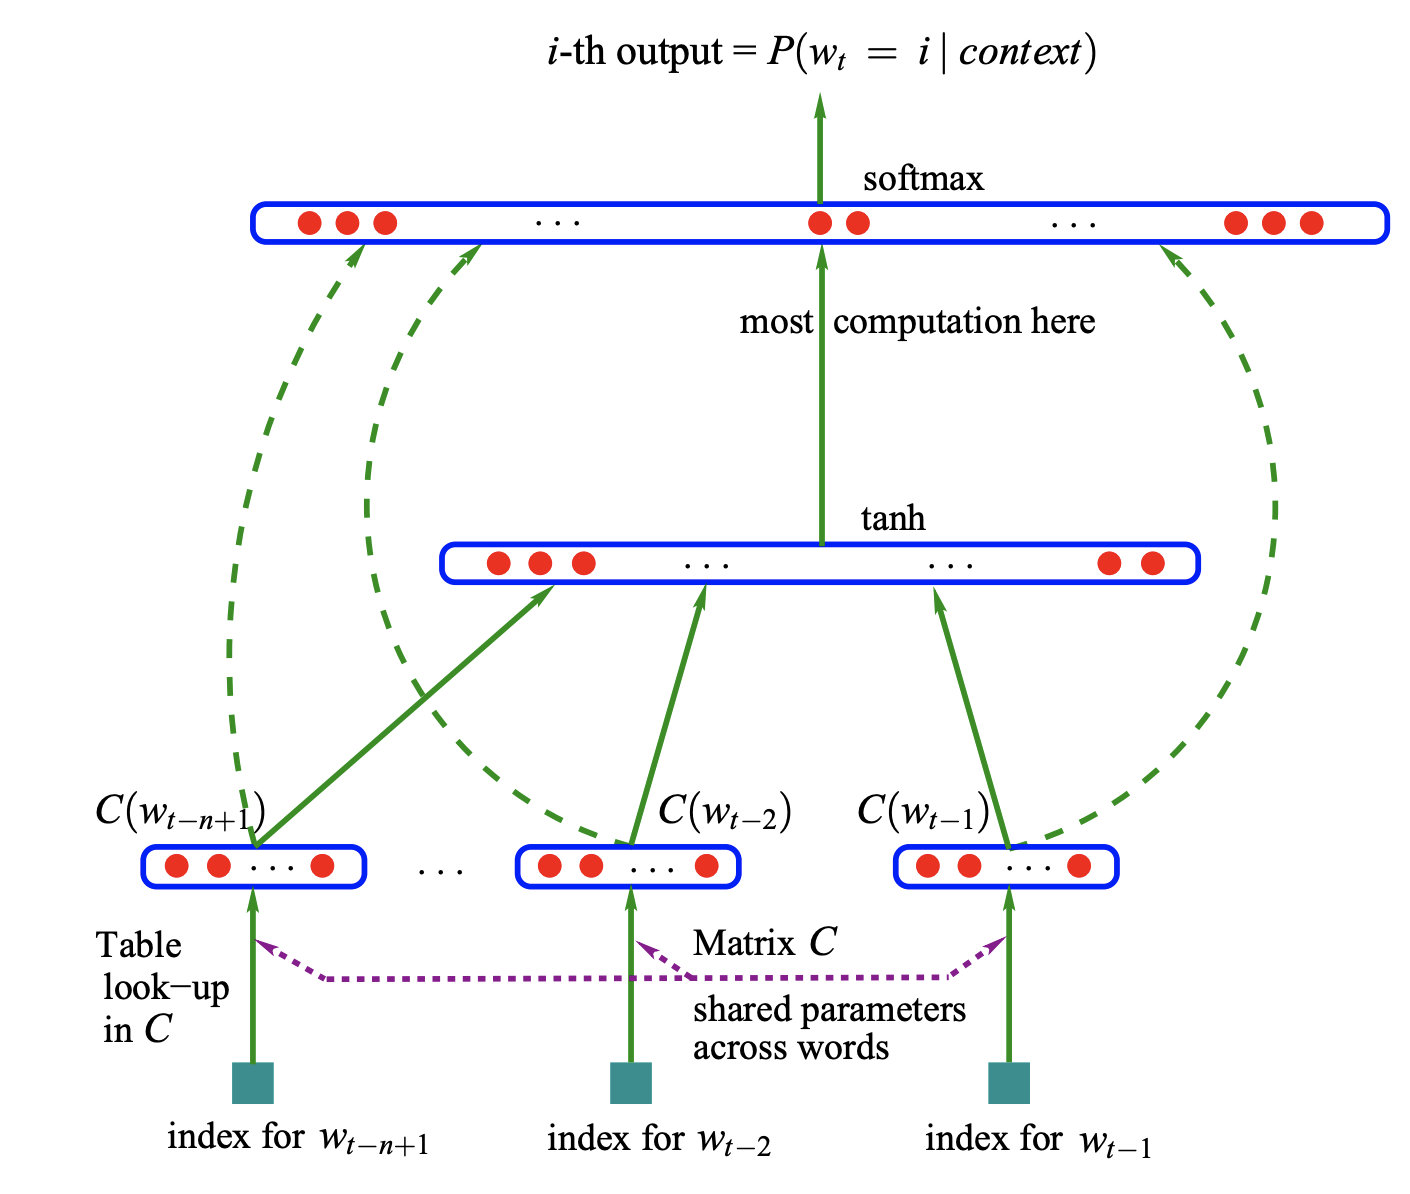
\includegraphics[width=\textwidth]{figures/bengio-2003-model.png}
    \caption{A pictorial depiction of the \ngram{} neural language model from the original publication \citep{Bengio2003}. Note that the quantity $C\left(w\right)$ corresponds to $\embedding_\sym$ for a word $\sym$ in our notation.}
    \label{fig:bengio-2003-model}
\end{figure}

This shows that the \ngram{} modeling framework is not limited to counting co-occurrence statistics. 
The model from \cref{eq:bengio-2003-model} can also be represented by a WFSA just like the simpler models we discussed above, with the weights on the transitions parametrized by the MLP.
This allows us to both understand well with insights from formal language theory, as well as to train it in a flexible way allowed for by the non-linear encoding function.
However, the model from \cref{eq:bengio-2003-model} is still limited to statistics of the last $\ngr$ tokens or less. 
If we want to model arbitrarily long dependencies and hierarchical structures, we have to leave the space of finite-state languages behind and develop formalisms capable of modeling more complex languages.
The next section explores the first of such frameworks, context-free languages with the computational models designed to model them.